\newpage
\chapter{Analysis}

Each feature of the word-vector model obtains its co-efficients from two separate sources:
\begin{itemize}
\item the first set of weights are trained in a similar fashion to the vanilla logistic regression model
\item the second set of weights are learnt by enforcing a word-vector regularization
\end{itemize}

We train the model as follows:\\

We initially keep word-vector weights constant at zero.
We then find the best model performance by training only the vanilla logistic regression model through extensive hyper-parameter tuning (l1/l2 regularization).

Once the vanilla feature weights have been learnt, we then start learning the word-vectors weights by increasing the l1/l2 regularization on the vanilla feature weights. This regularization would force the model to reduce the strength of the vanilla weights and move them to the unregularized word-vector weights. As the l1/l2 regularization strength per feature starts increasing, more and more weight from the vanilla model starts to shift onto the word-vector feature weights. 
The word-vector weights are constrained by a word-vector function. So when the word-vector model weights are substantial enough, then due to the word-vector similarity property, we are able to see the weights of the rare similar words also to start having a higher weight. This boosting of the rare word-weights would help improving the performance of the model.

However it is also possible that some labels better perform using the vanilla weights rather than the word-vector weights. In such a case, applying high regularization on the vanilla weights to boost the word-vector weights would be counterproductive. Thus, we need to perform extensive hyper-parameter tuning to find the right set of vanilla and word-vector weights that would work on all kinds of labels.\\

We performed several experiments to find the right set of hyper-parameters. Through these experiments we noticed that if the l1 penalty on the vanilla weights was too low, then the word-vector weights wouldn't increase much at all. They would remain almost close to zero. As we applied more and more l1 penalty, the model was forced to learn through the word-vector weights. 

Below is a graph showing various test results comparing l1 constraint per feature versus word-vector weights. We can see that the word-vector weights were increasing with higher L1 up to a certain point. After a certain threshold, the word-vector weights were almost non-increasing.

We also compared the model performance vs L1 strength. We can clearly see that the model performance increases initially with increasing L1 regularization and after a certain threshold, we see the model performance start to go down.\\\\

\begin{figure}[htbp]
\centering
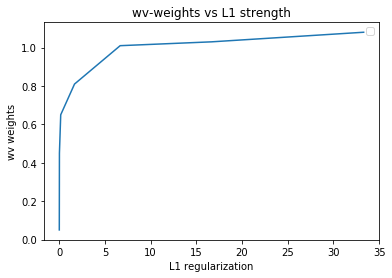
\includegraphics[width=16cm, height=10cm]{images/graph1.png}\\
\centering
\caption{Graph comparing word-vector weights with increasing L1 regularization}
\label{fig:graph1}
\end{figure}

\begin{figure}[htbp]
\centering
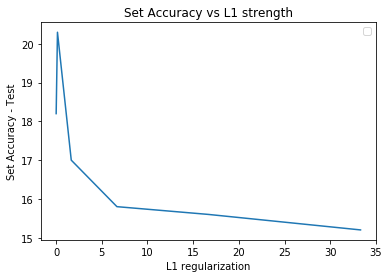
\includegraphics[width=16cm, height=10cm]{images/graph2.png}\\
\centering
\caption{Graph comparing model performance with increasing L1 regularization}
\label{fig:graph2}
\end{figure}


Upon comparing both models, we noticed that the performance of the word-vector models improved due to the additional word-vector weights.

To verify this, we took the top features for each model and printed the following:

\begin{itemize}
\item top similar words for each feature calculated based on the cosine similarity of the word-vectors

\item cosine similarity of the similar word

\item feature weight of the similar word

\item idf score of the similar word
\end{itemize}

The idf scores were computed to measure the rarity of the words. We noticed that the rare features which were similar to the important features now had similar weights. The below section shows such examples:

\newpage
\section{Examples of rare-similar words now having similar weights}

In this section we show a few examples where the word-vector model is able to generate similar weights for similar words, even if some of these words are rare. The rarity of the word can be determined by their corresponding Idf score. Due to the rarity of the words, the vanilla logistic regression model did not have enough information to determine the influence of these rare words and assigned them very small weights. However the word-vector models were able to assign comparatively higher weights due to their similarity feature.

\subsection{Example Case 1}

In the below example, we can see that \textbf{marijuana} and \textbf{narcotics} are rare features based on their higher Idf scores. Inspite of that, due to their similarity with the \textbf{drug}, they have substantially higher word-vector weights. Comparatively these rare words have very small weights when trained through vanilla logistic regression model. Thus, after using the word-vector model, when these rare words do appear in the test set, they now have a higher chance of getting classified under the class \textbf{Drug}.

\begin{table}[htbp]
\centering
\begin{tabular}{lllllll}
\multicolumn{7}{c}{\textbf{Class: Drugs}} \\ \hline
\multicolumn{1}{l|}{\textbf{}} & \multicolumn{1}{l|}{\textbf{Feature}} & \multicolumn{1}{l|}{\textbf{Similarity}} & \multicolumn{1}{l|}{\textbf{IDF}} & \multicolumn{1}{l|}{\textbf{Orig. $\theta_{lr}$}} & \multicolumn{1}{l|}{\textbf{New $\theta_{lr}$}} & \textbf{New $\theta_{wv}$} \\ \hline
\multicolumn{1}{l|}{\textbf{Top-feature}} & \multicolumn{1}{l|}{cannabis} & \multicolumn{1}{l|}{1} & \multicolumn{1}{l|}{5.5} & \multicolumn{1}{l|}{0.41} & \multicolumn{1}{l|}{0.39} & 0.16 \\ \hline
\multicolumn{1}{l|}{\textbf{Top-similar}} & \multicolumn{1}{l|}{\textbf{marijuana}} & \multicolumn{1}{l|}{\textbf{0.764}} & \multicolumn{1}{l|}{\textbf{6.0}} & \multicolumn{1}{l|}{\textbf{0.06}} & \multicolumn{1}{l|}{\textbf{0.01}} & \textbf{0.13} \\
\multicolumn{1}{l|}{\textbf{features}} & \multicolumn{1}{l|}{\textbf{cocaine}} & \multicolumn{1}{l|}{\textbf{0.694}} & \multicolumn{1}{l|}{\textbf{4.87}} & \multicolumn{1}{l|}{\textbf{0.20}} & \multicolumn{1}{l|}{\textbf{0.24}} & \textbf{0.13} \\
\multicolumn{1}{l|}{} & \multicolumn{1}{l|}{heroin} & \multicolumn{1}{l|}{0.671} & \multicolumn{1}{l|}{4.91} & \multicolumn{1}{l|}{0.19} & \multicolumn{1}{l|}{0.10} & 0.16 \\
\multicolumn{1}{l|}{\textbf{}} & \multicolumn{1}{l|}{\textbf{substances}} & \multicolumn{1}{l|}{\textbf{0.615}} & \multicolumn{1}{l|}{\textbf{5.69}} & \multicolumn{1}{l|}{\textbf{4e-4}} & \multicolumn{1}{l|}{\textbf{-1e-5}} & \textbf{0.07} \\
\multicolumn{1}{l|}{} & \multicolumn{1}{l|}{drug} & \multicolumn{1}{l|}{0.612} & \multicolumn{1}{l|}{3.28} & \multicolumn{1}{l|}{0.38} & \multicolumn{1}{l|}{0.27} & 0.16 \\
\multicolumn{1}{l|}{} & \multicolumn{1}{l|}{ecstasy} & \multicolumn{1}{l|}{0.601} & \multicolumn{1}{l|}{5.55} & \multicolumn{1}{l|}{0.14} & \multicolumn{1}{l|}{0.06} & 0.07 \\
\multicolumn{1}{l|}{\textbf{}} & \multicolumn{1}{l|}{\textbf{legalisation}} & \multicolumn{1}{l|}{\textbf{0.57}} & \multicolumn{1}{l|}{\textbf{6.59}} & \multicolumn{1}{l|}{\textbf{7e-4}} & \multicolumn{1}{l|}{\textbf{-2e-6}} & \textbf{0.05} \\
\multicolumn{1}{l|}{} & \multicolumn{1}{l|}{drugs} & \multicolumn{1}{l|}{0.567} & \multicolumn{1}{l|}{3.26} & \multicolumn{1}{l|}{0.40} & \multicolumn{1}{l|}{0.14} & 0.14 \\
\multicolumn{1}{l|}{} & \multicolumn{1}{l|}{tobacco} & \multicolumn{1}{l|}{0.559} & \multicolumn{1}{l|}{5.09} & \multicolumn{1}{l|}{-7e-4} & \multicolumn{1}{l|}{0.04} & 0.04 \\
\multicolumn{1}{l|}{\textbf{}} & \multicolumn{1}{l|}{\textbf{narcotics}} & \multicolumn{1}{l|}{\textbf{0.557}} & \multicolumn{1}{l|}{\textbf{6.19}} & \multicolumn{1}{l|}{\textbf{-4e-4}} & \multicolumn{1}{l|}{\textbf{0.06}} & \textbf{0.06}
\end{tabular}
\caption{\label{tab:widgets}Top feature weights comparison for cannabis}
\end{table}

\subsection{Example Case 2}

Here is an example which displays the vanilla and word-vector model weights for \textbf{chinese}, \textbf{shanghai} and \textbf{taiwan} which are some of the words used in similar context to \textbf{beijing}. Since \textbf{chinese} is not a rare word, we can see that its vanilla logistic regression model weight is quite high as compared to the word-vector model weight. However, when it comes across rarer words like \textbf{shanghai} and \textbf{taiwan}, its corresponding vanilla weights have dropped significantly, whereas the word-vector model weights are comparatively higher and closer to their corresponding word-vector weight of \textbf{beijing}. Also since the Olympics were held in \textbf{beijing} in 2008, both beijing and olympics have appeared in similar context and hence have similar word-vectors. Hence words like \textbf{olympics} and \textbf{olympic} also have high word-vector weights.

\begin{table}[htbp]
\centering
\begin{tabular}{lllllll}
\multicolumn{7}{c}{\textbf{Class: China}} \\ \hline
\multicolumn{1}{l|}{\textbf{}} & \multicolumn{1}{l|}{\textbf{Feature}} & \multicolumn{1}{l|}{\textbf{Similarity}} & \multicolumn{1}{l|}{\textbf{IDF}} & \multicolumn{1}{l|}{\textbf{Orig. $\theta_{lr}$}} & \multicolumn{1}{l|}{\textbf{New $\theta_{lr}$}} & \textbf{New $\theta_{lr}$} \\ \hline
\multicolumn{1}{l|}{\textbf{Top-feature}} & \multicolumn{1}{l|}{beijing} & \multicolumn{1}{l|}{1} & \multicolumn{1}{l|}{4.02} & \multicolumn{1}{l|}{0.373} & \multicolumn{1}{l|}{0.252} & 0.215 \\ \hline
\multicolumn{1}{l|}{\textbf{Top-similar}} & \multicolumn{1}{l|}{chinese} & \multicolumn{1}{l|}{0.696} & \multicolumn{1}{l|}{3.23} & \multicolumn{1}{l|}{0.388} & \multicolumn{1}{l|}{0.375} & 0.166 \\
\multicolumn{1}{l|}{\textbf{features}} & \multicolumn{1}{l|}{china} & \multicolumn{1}{l|}{0.68} & \multicolumn{1}{l|}{2.79} & \multicolumn{1}{l|}{0.78} & \multicolumn{1}{l|}{0.694} & 0.205 \\
\multicolumn{1}{l|}{} & \multicolumn{1}{l|}{\textbf{shanghai}} & \multicolumn{1}{l|}{\textbf{0.656}} & \multicolumn{1}{l|}{\textbf{5.17}} & \multicolumn{1}{l|}{\textbf{0.01}} & \multicolumn{1}{l|}{\textbf{0.075}} & \textbf{0.1} \\
\multicolumn{1}{l|}{\textbf{}} & \multicolumn{1}{l|}{\textbf{taiwan}} & \multicolumn{1}{l|}{\textbf{0.606}} & \multicolumn{1}{l|}{\textbf{5.53}} & \multicolumn{1}{l|}{\textbf{9e-4}} & \multicolumn{1}{l|}{\textbf{3e-5}} & \textbf{0.073} \\
\multicolumn{1}{l|}{} & \multicolumn{1}{l|}{\textbf{olympics}} & \multicolumn{1}{l|}{\textbf{0.602}} & \multicolumn{1}{l|}{\textbf{4.2}} & \multicolumn{1}{l|}{\textbf{0.002}} & \multicolumn{1}{l|}{\textbf{2e-5}} & \textbf{0.146} \\
\multicolumn{1}{l|}{} & \multicolumn{1}{l|}{tibet} & \multicolumn{1}{l|}{0.6} & \multicolumn{1}{l|}{5.66} & \multicolumn{1}{l|}{0.002} & \multicolumn{1}{l|}{7e-5} & 0.09 \\
\multicolumn{1}{l|}{\textbf{}} & \multicolumn{1}{l|}{\textbf{olympic}} & \multicolumn{1}{l|}{\textbf{0.543}} & \multicolumn{1}{l|}{\textbf{4.28}} & \multicolumn{1}{l|}{\textbf{0.049}} & \multicolumn{1}{l|}{\textbf{-1e-5}} & \textbf{0.15} \\
\multicolumn{1}{l|}{} & \multicolumn{1}{l|}{singapore} & \multicolumn{1}{l|}{0.534} & \multicolumn{1}{l|}{5.19} & \multicolumn{1}{l|}{2e-4} & \multicolumn{1}{l|}{-1e-5} & 0.014 \\
\multicolumn{1}{l|}{} & \multicolumn{1}{l|}{tokyo} & \multicolumn{1}{l|}{0.503} & \multicolumn{1}{l|}{4.69} & \multicolumn{1}{l|}{0.503} & \multicolumn{1}{l|}{-1e-5} & 0.036 \\
\multicolumn{1}{l|}{\textbf{}} & \multicolumn{1}{l|}{korea} & \multicolumn{1}{l|}{0.498} & \multicolumn{1}{l|}{4.26} & \multicolumn{1}{l|}{-3e-4} & \multicolumn{1}{l|}{1e-4} & 0.031
\end{tabular}
\caption{\label{tab:widgets}Top feature weights comparison for beijing}
\end{table}


\subsection{Example Case 3}

Below is a similar example where \textbf{ranch} is a top feature for the class \textbf{Western}. Again we can see that the weights of rare-words \textbf{cattle}, \textbf{farm} and \textbf{sheep} have been boosted due to the word-vector model.

\begin{table}[htbp]
\centering
\begin{tabular}{lllllll}
\multicolumn{7}{c}{\textbf{Class: Western}} \\ \hline
\multicolumn{1}{l|}{\textbf{}} & \multicolumn{1}{l|}{\textbf{Feature}} & \multicolumn{1}{l|}{\textbf{Similarity}} & \multicolumn{1}{l|}{\textbf{IDF}} & \multicolumn{1}{l|}{\textbf{Orig. $\theta_{lr}$}} & \multicolumn{1}{l|}{\textbf{New $\theta_{lr}$}} & \textbf{New $\theta_{lr}$} \\ \hline
\multicolumn{1}{l|}{\textbf{Top-feature}} & \multicolumn{1}{l|}{ranch} & \multicolumn{1}{l|}{1} & \multicolumn{1}{l|}{5.29} & \multicolumn{1}{l|}{0.371} & \multicolumn{1}{l|}{0.104} & 1.217 \\ \hline
\multicolumn{1}{l|}{\textbf{Top-similar}} & \multicolumn{1}{l|}{\textbf{cattle}} & \multicolumn{1}{l|}{\textbf{0.716}} & \multicolumn{1}{l|}{\textbf{5.55}} & \multicolumn{1}{l|}{\textbf{0.34}} & \multicolumn{1}{l|}{\textbf{0.05}} & \textbf{0.878} \\
\multicolumn{1}{l|}{\textbf{features}} & \multicolumn{1}{l|}{\textbf{farm}} & \multicolumn{1}{l|}{\textbf{0.705}} & \multicolumn{1}{l|}{\textbf{4.24}} & \multicolumn{1}{l|}{\textbf{3e-4}} & \multicolumn{1}{l|}{\textbf{4e-5}} & \textbf{0.486} \\
\multicolumn{1}{l|}{} & \multicolumn{1}{l|}{rancher} & \multicolumn{1}{l|}{0.702} & \multicolumn{1}{l|}{5.96} & \multicolumn{1}{l|}{0.001} & \multicolumn{1}{l|}{-4e-5} & 0.844 \\
\multicolumn{1}{l|}{\textbf{}} & \multicolumn{1}{l|}{\textbf{cowboy}} & \multicolumn{1}{l|}{\textbf{0.626}} & \multicolumn{1}{l|}{\textbf{5.71}} & \multicolumn{1}{l|}{\textbf{-5e-6}} & \multicolumn{1}{l|}{\textbf{-1e-5}} & \textbf{0.722} \\
\multicolumn{1}{l|}{} & \multicolumn{1}{l|}{farmer} & \multicolumn{1}{l|}{0.606} & \multicolumn{1}{l|}{5.04} & \multicolumn{1}{l|}{0.001} & \multicolumn{1}{l|}{-4e-5} & 0.404 \\
\multicolumn{1}{l|}{} & \multicolumn{1}{l|}{\textbf{sheep}} & \multicolumn{1}{l|}{\textbf{0.591}} & \multicolumn{1}{l|}{\textbf{6.03}} & \multicolumn{1}{l|}{\textbf{1e-4}} & \multicolumn{1}{l|}{\textbf{-3e-5}} & \textbf{0.314} \\
\multicolumn{1}{l|}{\textbf{}} & \multicolumn{1}{l|}{plantation} & \multicolumn{1}{l|}{0.59} & \multicolumn{1}{l|}{6.23} & \multicolumn{1}{l|}{8e-4} & \multicolumn{1}{l|}{-2e-6} & 0.085 \\
\multicolumn{1}{l|}{} & \multicolumn{1}{l|}{\textbf{texas}} & \multicolumn{1}{l|}{\textbf{0.579}} & \multicolumn{1}{l|}{\textbf{4.67}} & \multicolumn{1}{l|}{\textbf{0.003}} & \multicolumn{1}{l|}{\textbf{-1e-5}} & \textbf{0.919} \\
\multicolumn{1}{l|}{} & \multicolumn{1}{l|}{county} & \multicolumn{1}{l|}{0.579} & \multicolumn{1}{l|}{5.3} & \multicolumn{1}{l|}{6e-4} & \multicolumn{1}{l|}{-3e-5} & 0.025 \\
\multicolumn{1}{l|}{\textbf{}} & \multicolumn{1}{l|}{farmhouse} & \multicolumn{1}{l|}{0.578} & \multicolumn{1}{l|}{6.07} & \multicolumn{1}{l|}{1e-4} & \multicolumn{1}{l|}{-4e-6} & 0.051
\end{tabular}
\caption{\label{tab:widgets}Top feature weights comparison for ranch}
\end{table}


The above examples do help in proving that our model was successfully able to use word-vectors as a regularizer to assign similar weights to similar words even if those similar words happen to be rare.

\newpage
\section{Scenarios when word-vector model doesn't work}

In this section we show an example that highlights the major drawback of word-vectors - they presume that a word's meaning is stable across sentences. As we know this approach to word representation does not address the co-existence of many possible meanings for a given word or phrase.

\subsection{Example Case 1}

From the below example, we can see \textbf{west} is one of the top feature for the class \textbf{Western} and it has high vanilla and word-vector weights. However since the word-vectors consider west as a direction(noun), other directions which are used in similar contexts now have higher word-vector weights. So when any of the features such as \textbf{north}, \textbf{east} or \textbf{south} appear in the train or testset, there is a higher chance the word-vector model may misclassify the document to belong to the \textbf{Western} class leading to more false positives. Out of all the top most similar features to west, \textbf{texas} is the only feature which is more relevant to the class we are trying to predict. We do observe expected performance from the word-vector model generating high word-vector weights even though its vanilla weights are negligible.

\begin{table}[htbp]
\centering
\begin{tabular}{lllllll}
\multicolumn{7}{c}{\textbf{Class: Western}} \\ \hline
\multicolumn{1}{l|}{\textbf{}} & \multicolumn{1}{l|}{\textbf{Feature}} & \multicolumn{1}{l|}{\textbf{Similarity}} & \multicolumn{1}{l|}{\textbf{IDF}} & \multicolumn{1}{l|}{\textbf{Orig. $\theta_{lr}$}} & \multicolumn{1}{l|}{\textbf{New $\theta_{lr}$}} & \textbf{New $\theta_{lr}$} \\ \hline
\multicolumn{1}{l|}{\textbf{Top-feature}} & \multicolumn{1}{l|}{west} & \multicolumn{1}{l|}{1} & \multicolumn{1}{l|}{3.95} & \multicolumn{1}{l|}{1.63} & \multicolumn{1}{l|}{0.224} & 0.98 \\ \hline
\multicolumn{1}{l|}{\textbf{Top-similar}} & \multicolumn{1}{l|}{north} & \multicolumn{1}{l|}{0.823} & \multicolumn{1}{l|}{4.06} & \multicolumn{1}{l|}{-8e-4} & \multicolumn{1}{l|}{-4e-5} & 0.38 \\
\multicolumn{1}{l|}{\textbf{features}} & \multicolumn{1}{l|}{east} & \multicolumn{1}{l|}{0.822} & \multicolumn{1}{l|}{4.26} & \multicolumn{1}{l|}{0.117} & \multicolumn{1}{l|}{-3e-5} & 0.297 \\
\multicolumn{1}{l|}{} & \multicolumn{1}{l|}{south} & \multicolumn{1}{l|}{0.821} & \multicolumn{1}{l|}{3.72} & \multicolumn{1}{l|}{0.016} & \multicolumn{1}{l|}{5e-5} & 0.233 \\
\multicolumn{1}{l|}{\textbf{}} & \multicolumn{1}{l|}{southwestern} & \multicolumn{1}{l|}{0.731} & \multicolumn{1}{l|}{6.75} & \multicolumn{1}{l|}{7e-4} & \multicolumn{1}{l|}{1e-5} & 0.098 \\
\multicolumn{1}{l|}{} & \multicolumn{1}{l|}{northwestern} & \multicolumn{1}{l|}{0.704} & \multicolumn{1}{l|}{6.93} & \multicolumn{1}{l|}{3e-4} & \multicolumn{1}{l|}{1e-5} & 0.123 \\
\multicolumn{1}{l|}{} & \multicolumn{1}{l|}{southern} & \multicolumn{1}{l|}{0.688} & \multicolumn{1}{l|}{4.77} & \multicolumn{1}{l|}{-0.24} & \multicolumn{1}{l|}{-3e-5} & 0.308 \\
\multicolumn{1}{l|}{\textbf{}} & \multicolumn{1}{l|}{eastern} & \multicolumn{1}{l|}{0.633} & \multicolumn{1}{l|}{5.14} & \multicolumn{1}{l|}{5e-4} & \multicolumn{1}{l|}{2e-5} & -0.015 \\
\multicolumn{1}{l|}{} & \multicolumn{1}{l|}{northern} & \multicolumn{1}{l|}{0.633} & \multicolumn{1}{l|}{4.94} & \multicolumn{1}{l|}{-0.001} & \multicolumn{1}{l|}{1e-5} & 0.022 \\
\multicolumn{1}{l|}{} & \multicolumn{1}{l|}{central} & \multicolumn{1}{l|}{0.614} & \multicolumn{1}{l|}{4.76} & \multicolumn{1}{l|}{-0.194} & \multicolumn{1}{l|}{-4e-5} & -0.075 \\
\multicolumn{1}{l|}{\textbf{}} & \multicolumn{1}{l|}{\textbf{texas}} & \multicolumn{1}{l|}{\textbf{0.612}} & \multicolumn{1}{l|}{\textbf{4.67}} & \multicolumn{1}{l|}{\textbf{1.91}} & \multicolumn{1}{l|}{\textbf{-1e-5}} & \textbf{0.919}
\end{tabular}
\caption{\label{tab:widgets}Top feature weights comparison for west}
\end{table}

\newpage
\section{Scenarios when word-vector model works because of word-vector coefficients not because of similarity}

In this section we look at a few more examples of polysemy - same word having different meaning. For such cases we were expecting the corresponding word-vector weights to be high for similar but non-relevant words. But since the word-vector weights were trained on a specific dataset, they managed to train the word-vector coefficients in such a way that similar but non-relevant words got an almost zero word-vector weight.

\subsection{Example Case 1}

Below is one of the top feature \textbf{amazon} trained for the label \textbf{Brazil}. Here \textbf{amazon}  refers to the largest river in South America that flows through \textbf{Brazil}. It does not refer to the multinational technology company Amazon that focuses on e-commerce and digital streaming. However as seen below the top words for amazon are kindle, ebooks, itunes and download. These top words are however are relevant to the classfication problem we're trying to solve in this case. One may expect the word-vector model to generate similar weights for these words, but since the 300 dimensional word-vector coefficients were trained on this particular label, we see that it managed to assign the weights in such a way that these non-relevant words have an almost zero word-vector weight.

We can also see that \textbf{rainforest} is the only relevant word that is more relevant to this context and it got a higher word-vector weight even tough it had much lower similarity to amazon as compared to the other words like kindle, ebooks etc.

\begin{table}[htbp]
\centering
\begin{tabular}{lllllll}
\multicolumn{7}{c}{\textbf{Class: Brazil}} \\ \hline
\multicolumn{1}{l|}{\textbf{}} & \multicolumn{1}{l|}{\textbf{Feature}} & \multicolumn{1}{l|}{\textbf{Similarity}} & \multicolumn{1}{l|}{\textbf{IDF}} & \multicolumn{1}{l|}{\textbf{Orig. $\theta_{lr}$}} & \multicolumn{1}{l|}{\textbf{New $\theta_{lr}$}} & \textbf{New $\theta_{lr}$} \\ \hline
\multicolumn{1}{l|}{\textbf{Top-feature}} & \multicolumn{1}{l|}{amazon} & \multicolumn{1}{l|}{1} & \multicolumn{1}{l|}{4.3} & \multicolumn{1}{l|}{0.154} & \multicolumn{1}{l|}{-3e-5} & 0.202 \\ \hline
\multicolumn{1}{l|}{\textbf{Top-similar}} & \multicolumn{1}{l|}{kindle} & \multicolumn{1}{l|}{0.699} & \multicolumn{1}{l|}{5.96} & \multicolumn{1}{l|}{-4e-4} & \multicolumn{1}{l|}{-8e-6} & 0.06 \\
\multicolumn{1}{l|}{\textbf{features}} & \multicolumn{1}{l|}{ebooks} & \multicolumn{1}{l|}{0.655} & \multicolumn{1}{l|}{6.51} & \multicolumn{1}{l|}{4e-4} & \multicolumn{1}{l|}{-6e-5} & 0.011 \\
\multicolumn{1}{l|}{} & \multicolumn{1}{l|}{ebook} & \multicolumn{1}{l|}{0.643} & \multicolumn{1}{l|}{6.38} & \multicolumn{1}{l|}{-9e-4} & \multicolumn{1}{l|}{6e-6} & 0.2 \\
\multicolumn{1}{l|}{\textbf{}} & \multicolumn{1}{l|}{itunes} & \multicolumn{1}{l|}{0.628} & \multicolumn{1}{l|}{4.8} & \multicolumn{1}{l|}{2e-4} & \multicolumn{1}{l|}{-6e-5} & 5e-5 \\
\multicolumn{1}{l|}{} & \multicolumn{1}{l|}{ebay} & \multicolumn{1}{l|}{0.598} & \multicolumn{1}{l|}{5.08} & \multicolumn{1}{l|}{-3e-4} & \multicolumn{1}{l|}{-2e-5} & 0.015 \\
\multicolumn{1}{l|}{} & \multicolumn{1}{l|}{downloads} & \multicolumn{1}{l|}{0.584} & \multicolumn{1}{l|}{4.85} & \multicolumn{1}{l|}{-7e-4} & \multicolumn{1}{l|}{6e-5} & -8e-4 \\
\multicolumn{1}{l|}{\textbf{}} & \multicolumn{1}{l|}{google} & \multicolumn{1}{l|}{0.555} & \multicolumn{1}{l|}{3.12} & \multicolumn{1}{l|}{-1e-3} & \multicolumn{1}{l|}{2e-5} & -.04 \\
\multicolumn{1}{l|}{} & \multicolumn{1}{l|}{download} & \multicolumn{1}{l|}{0.54} & \multicolumn{1}{l|}{3.95} & \multicolumn{1}{l|}{4e-4} & \multicolumn{1}{l|}{-5e-5} & 3e-2 \\
\multicolumn{1}{l|}{} & \multicolumn{1}{l|}{paypal} & \multicolumn{1}{l|}{0.531} & \multicolumn{1}{l|}{6.5} & \multicolumn{1}{l|}{3e-4} & \multicolumn{1}{l|}{-6e-5} & 0.02 \\
\multicolumn{1}{l|}{\textbf{}} & \multicolumn{1}{l|}{\textbf{rainforest}} & \multicolumn{1}{l|}{\textbf{0.52}} & \multicolumn{1}{l|}{\textbf{5.33}} & \multicolumn{1}{l|}{\textbf{-2e-4}} & \multicolumn{1}{l|}{\textbf{4e-5}} & \textbf{0.167}
\end{tabular}
\caption{\label{tab:widgets}Top feature weights comparison for amazon}
\end{table}

\iffalse
\newpage
\subsection{Example Case 2}

\begin{table}[htbp]
\begin{tabular}{llllll}
\multicolumn{2}{l|}{\textbf{Class: Crime}}                                   & \multicolumn{1}{l|}{\textbf{\begin{tabular}[c]{@{}l@{}}vanilla\\ weights\end{tabular}}} & \multicolumn{1}{l|}{\textbf{Similarity}} & \multicolumn{1}{l|}{\textbf{Idf-score}} & \textbf{\begin{tabular}[c]{@{}l@{}}wv\\ weights\end{tabular}} \\ \hline
\multicolumn{1}{l|}{\textbf{Top-feature}} & \multicolumn{1}{l|}{examination} & \multicolumn{1}{l|}{1.5}                                                                & \multicolumn{1}{l|}{1}                   & \multicolumn{1}{l|}{5.63}               & 0.245                                                         \\ \hline
\multicolumn{1}{l|}{\textbf{Top similar}} & \multicolumn{1}{l|}{tests}       & \multicolumn{1}{l|}{1e-4}                                                               & \multicolumn{1}{l|}{0.698}               & \multicolumn{1}{l|}{5.53}               & 0.003                                                         \\
\multicolumn{1}{l|}{\textbf{features}}    & \multicolumn{1}{l|}{exam}        & \multicolumn{1}{l|}{1e-5}                                                               & \multicolumn{1}{l|}{0.646}               & \multicolumn{1}{l|}{6.55}               & 0.010                                                         \\
\multicolumn{1}{l|}{}                     & \multicolumn{1}{l|}{analysis}    & \multicolumn{1}{l|}{0.496}                                                              & \multicolumn{1}{l|}{0.642}               & \multicolumn{1}{l|}{6.93}               & 0.21                                                          \\
                                          &                                  &                                                                                         &                                          &                                         &                                                              
\end{tabular}
\end{table}
\fi